\documentclass[a4paper,10pt]{scrartcl}

\usepackage{units}
\usepackage{mathtools}
%\usepackage{a4wide}
\usepackage{bbm}
\usepackage{amssymb}
\usepackage{amsthm}
\usepackage{amsmath}
\usepackage{graphicx, enumerate}
\usepackage{psfrag}
\usepackage[matrix, arrow, curve]{xy}
\usepackage{array,tabularx}
%\usepackage[square, comma, numbers]{natbib}
\usepackage[unicode, a4paper]{hyperref}
\usepackage{subfigure}
\usepackage{algorithm2e}
\usepackage{url}
\usepackage{mathtools}
\usepackage{pgfplots}
\usepackage{siunitx}

\newcounter{myFCounter}[section]
\newcommand{\myFigure}[3]{%
    \begin{center}\begin{minipage}[t]{\columnwidth}%
    \begin{center}\refstepcounter{myFCounter}\vspace{1ex}%
    \includegraphics[width=#1\columnwidth,keepaspectratio]{#2}\ \\%
     Abb. \arabic{myFCounter}:\ \rm #3 
    \vspace{1ex}\end{center}%
    \end{minipage}\end{center}}
    \newcommand\myColumnSep[1]{%
\setlength{\columnsep}{#1}%
}

\newcommand{\inner}[2]{\left\langle #1, #2 \right\rangle}
\newcommand{\abs}[1]{\left| #1 \right|}

%die folgenden Zeilen sind für die Kopf und Fusszeile
%die eckigen Klammern betreffen die Titelseite, die geschwungenen Klammern das restliche Dokument 
\usepackage[automark]{scrpage2}
\pagestyle{scrheadings}
\ihead{
\includegraphics[width=0.25 \textwidth]{figures/NTB-FHO_LOGO_2}} % linke Kopfzeile 
\chead{Estimating Outdoor Signal Strength of LoRaWAN} % mittlere Kopfzeile
\ohead{
\includegraphics[width=0.15 \textwidth]{figures/logo_thingslogic}} % rechte Kopfzeile
%\cfoot[...]{\thepage} % mittlere Fusszeile 
\ofoot[...]{\today} % rechte Fusszeile 
\ifoot[...]{} 
\setheadsepline{0.5pt}
\setfootsepline{0.5pt}
%Befehle für kopf und fusszeile fertig

\setlength{\parindent}{0pt}
\setlength{\footskip}{1cm}

\linespread{1.5} %Für Zeilenabstand 1.5 muss linespreadfaktor auf 1.25 eingestellt werden.
%\onehalfspacing%Zeilenabstand (alternativ zu linespread

% Zeilenabstand verringern bei itemize
\let\origitemize\itemize
\def\itemize{\origitemize\itemsep0pt}
\setlength{\topmargin}{-1.5cm}  		%	Abstand Seitenkopf vom oberen Rand plus 1 Inch
\setlength{\textwidth}{17cm} 				%	{6.25in}  %Breite des Seitenrumpfes (15.8cm)
\setlength{\oddsidemargin}{-0.5cm}	%	{0in} %Abstand Text vom linken Rand plus ein Inch (=2.54cm)
\setlength{\textheight}{9.0in}  		%	Texthöhe ohne Kopfzeile und Fusszeile (23.9cm)
\setlength{\headheight}{1.3cm}			%	Kopfzeilenhöhe
\setlength{\headsep}{0.5cm}				%	Abstand Kopfzeile - Text
%\setlength{\headsep}{1cm}						%	Abstand Kopfzeile - Text
\setlength{\columnsep}{.5cm}				%	Abstand der 2 Kolonnen
%
\pagestyle{scrheadings}							%	Einzug bei Absatzbeginn unterdrücken

%\renewcommand{\figurename}{Abb.}		%	Text zur Bildbeschriftung
%\renewcommand{\tablename}{Tab.}			%	Text zur Tabellenbeschriftung
%\renewcommand{\refname}{Literaturverzeichnis}
%\let\mathmu\mu
%\def\mu{\ensuremath{\mathmu}}

\usepackage{tikz}
\usetikzlibrary{calc}
\usetikzlibrary{patterns}
%\usetikzlibrary{angles,quotes}



% theoremstyles 
\theoremstyle{plain}

\newtheorem{thm}{Theorem}[section]
\newtheorem{prop}[thm]{Proposition}
\newtheorem{ass}[thm]{Assumption}

\newtheorem{assa}{Assumption}
\renewcommand{\theassa}{\Alph{assa}}

\theoremstyle{definition}
\newtheorem{rem}[thm]{Remark}
\newtheorem{alg}[thm]{Algorithm}
\newtheorem{lem}[thm]{Lemma}
\newtheorem{dfn}[thm]{Definition}
\newtheorem{cor}[thm]{Corollary}
\newtheorem{que}{Question}
\newtheorem{example}[thm]{Example}
\newtheorem*{example*}{Example}

\newtheorem*{dfn*}{Definition}
\newtheorem*{alg*}{Algorithm}



\theoremstyle{remark}
\newtheorem{prob}{Problem}



\pgfplotsset{compat=1.11}
\begin{document}
%********************************************************************************************************************************************
% Titelseite %********************************************************************************************************************************************
\thispagestyle{empty}

\pagestyle{scrheadings}
\setlength{\headsep}{1.5cm}					%Abstand Kopfzeile - Text
\begin{tabularx}{\textwidth}{lXr}
	
\includegraphics[height=2.2cm]{figures/NTB-FHO_LOGO_2} & & 
\includegraphics[height=2.2cm]{figures/logo_thingslogic}
\end{tabularx}

\begin{center}
	\vspace{5cm}
	\textsf{\huge Estimating Outdoor Signal Strength of LoRaWAN with Regression Kriging} \\
	\vspace{0.5cm}	
	{\textsf{\large Final Report: FFG Innovationsscheck 864448} \par}
	\vspace{0.5cm}
%	\textsf{\Large mittels makroskopischer Modellierung der konzentrierten Suspension} \\
%	\vspace{1.5cm}
%	\begin{figure}[H]
%	\centering
%	\begin{tikzpicture}
%	\draw (0,0) node{\includegraphics[width=0.6\textwidth]{Bilder/Titelbild_Neu}};
%	%\draw(0,-3.6) node{\scriptsize $t=0\,$s};
%	%\draw (4.2,0) node{\includegraphics[width=1cm]{Bilder/Titelbild2}};
%	%\draw (8,0) node{\includegraphics[width=0.3\textwidth]{Bilder/Titelbild}};
%	%\draw(8,-3.6) node{\scriptsize $t=100\,$s};
%	\end{tikzpicture}
%	\end{figure}
	\vspace{1.5cm}
	\textsf{\Large Christian Anselmi, Josef B\"ockle, Klaus Frick } \\
	\vspace{8.5cm}
	\textsf{\Large ThingsLogic} \\
	\textsf{\Large  Institut f\"ur Computational Engineering ICE, NTB} \\
\end{center}
\vspace{2.5cm}








\section{Introduction}\label{sec:intro}

In the emerging field of Internet of Things (IoT) the paradigm of connecting literally any object to the internet is a key feature. Establishing an everyday life filled with wireless devices improving the aspects of our existence, however, imposes several requirements on these systems: long battery life, low price of devices and long-range coverage (\cite{Nolan2016, Augustin2016}).  LoRaWAN is a low-power wide-area network (LPWAN) protocol that accounts for the last requirement. It stands for Long Range Wide Area Network and is an open standard maintained by the LoRa Alliance (\cite{LoRaAlliance2015}). LoRa is the physical layer of the protocol. It is based on the Chirp Spread Spectrum (CSS) modulation technique and uses the ISM band between 863-870 MHz in Europe. 

The topology of a LoRaWAN  is sketched in Figure \ref{fig:loraarch}. Several IoT devices send and receive data via the LoRaWAN protocol to and from one or more gateways simultaneously in a single hop. From there, all packages are forwarded to a network server via standard TCP/IP. The data can then be disaggregated and used for specific applications. The devices are identified by a unique ID, which is registered in the network server. There are several network provider as for example the open source project The Things Network (TTN).

\begin{figure}[h!]
\centering
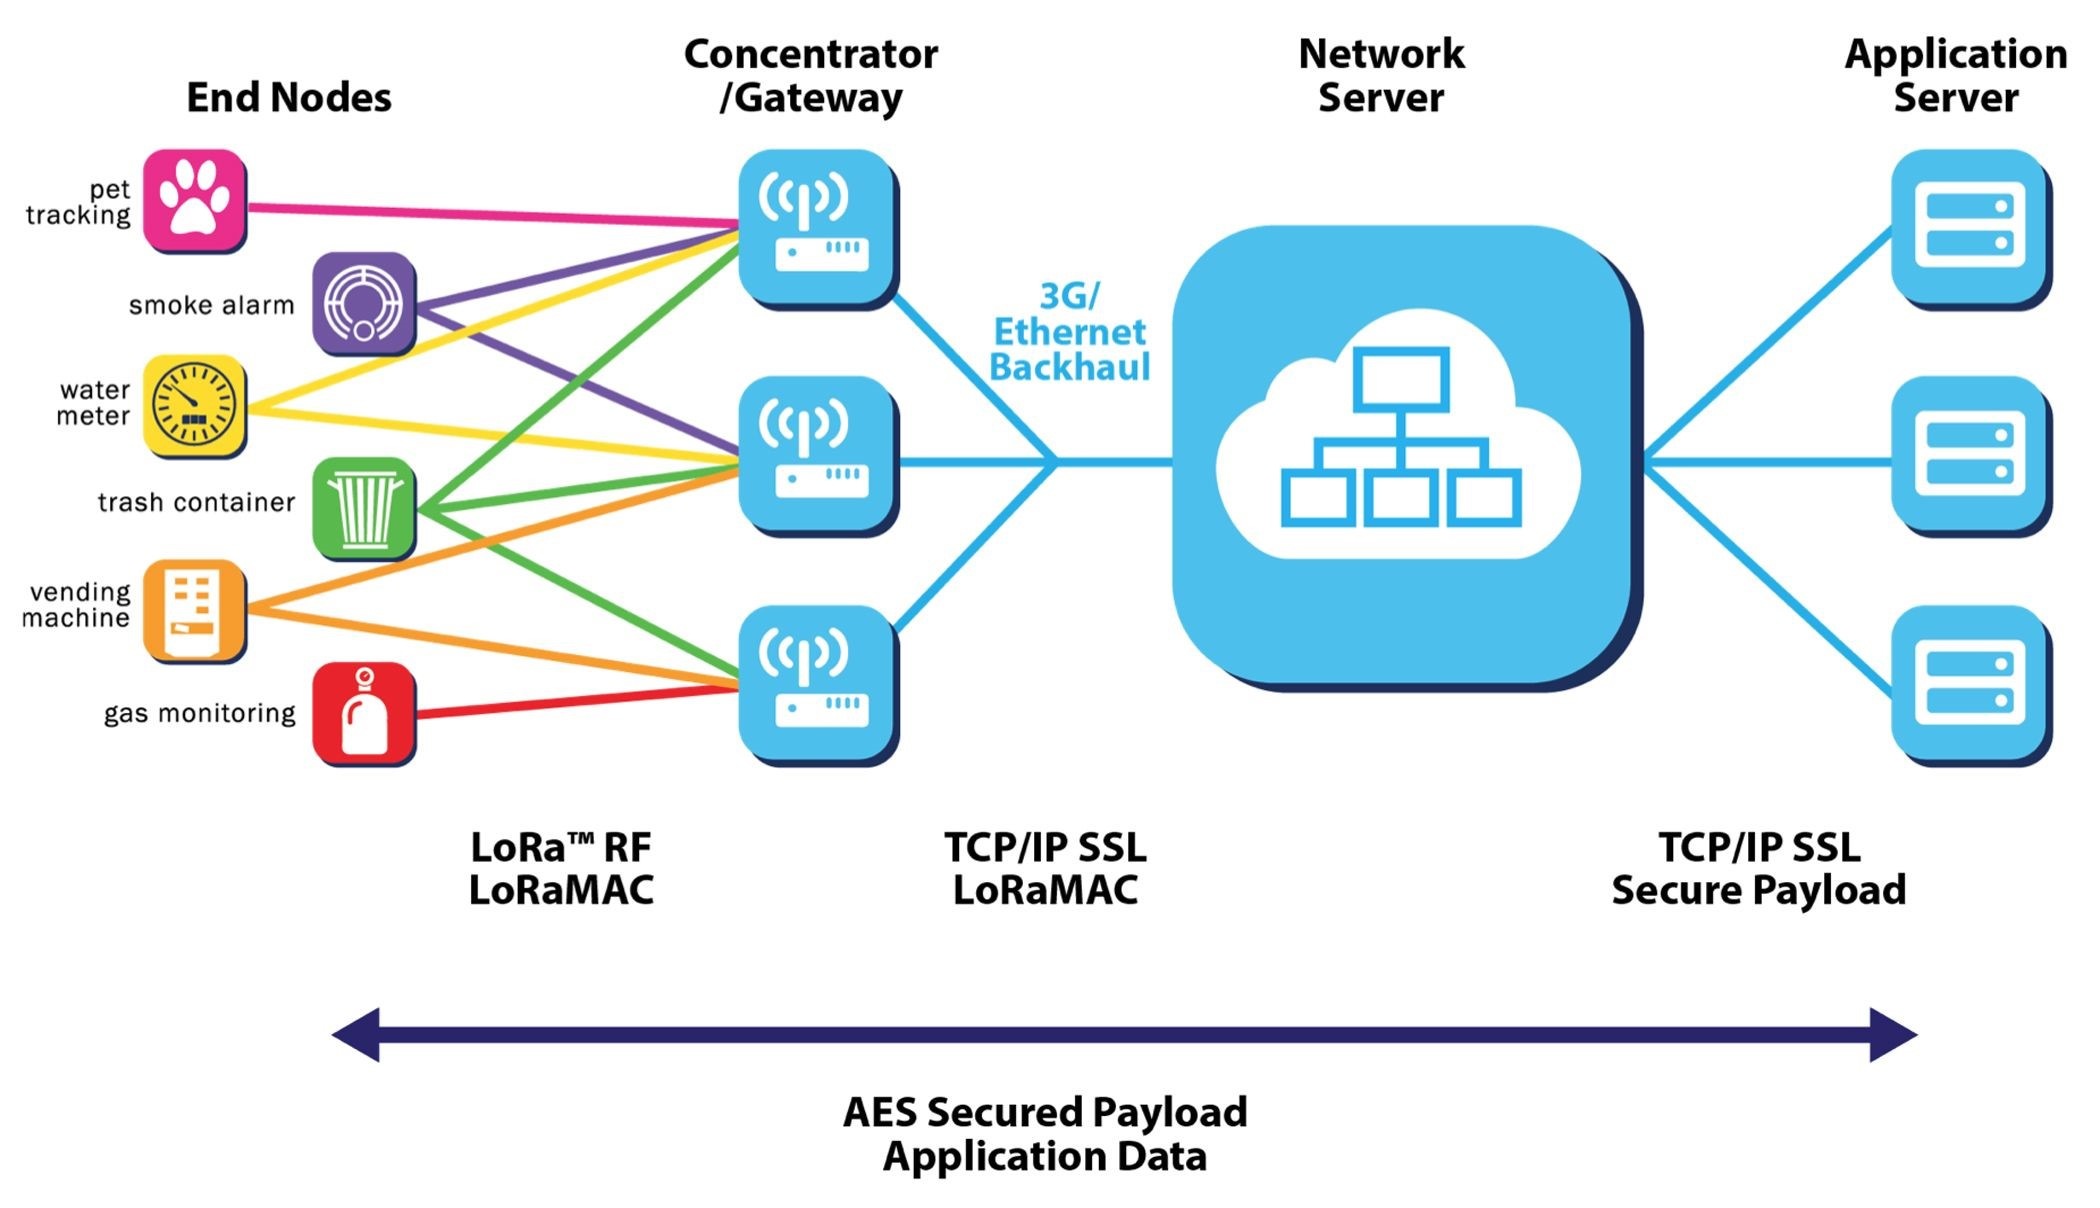
\includegraphics[width=0.7\textwidth]{figures/LoRa_Arch}
\caption{LoRa WAN Topology (taken from \cite{LoRaAlliance2015}).}\label{fig:loraarch}
\end{figure}

Due to the prime requirement of long range data transmission, field tests for LoRaWAN are mainly concerned with assessing signal strength and quality in dependence of the distance between device and gateway. There, different quality measures are studied (cf. \cite{Aref2014, Marais2017, }).
\begin{enumerate}
\item The Receiver Signal Strength Indicator (RSSI) ) is the total signal power received in milliwatts. The RSSI  is  measured  in  the  decibel-milliwatts  (dBm).
\item The Signal-to-Noise ratio (SNR) is  a  ratio  between  the  level  of  the  signal  and  the  level  of noise.
\item The packet-loss refers to frames that are not received by the network server. Such frames can be either not received at all by the gateway or received by the gateway but with a bad CRC (Cyclic Redundancy Check) so they can not be decoded.
\end{enumerate}

In this work we focus on the RSSI as quality measure of the network coverage. Under ideal conditions, the RSSI value has a logarithmic dependence on the distance $d$ of the device to the gateway, i.e.
\begin{equation}\label{eqn:loglaw}
\text{RSSI} = A -B \log_{10}(d)
\end{equation}
for some constants $A$ and $B$. In practice, however, the decay of signal strength also heavily depends on localized effects such as the surrounding elevation, environmental influences as well as buildings and vegetation that loom in the Fresnel zone of the device/gateway pair.   

In order to generate a reliable heat map that predicts the RSSI values between measurement points, we employ techniques from geospatial statistics (cf. \cite{Cressi1993, Webster2007}). In particular, we use regression kriging that allows for the spatial variance structure of the measurements and hence yields RSSI predictions that are sensitive to localized effects. In our situation, regression kriging amounts to update the predictions of the logarithmic regression model above with spatially interpolated residuals that take into account the covariance structure of the neighborhood of the spatial point under consideration.  

The contribution of this work is threefold:
\begin{enumerate}
\item 
\end{enumerate}

\section{Measurement Setup}\label{sec:setup}

The mobile measuring device is a simple assembly of commodity electronic items with a light-weight code. The device consists of
\begin{itemize}
\item An Arduino Mega 2560 R3 microcontroller board.
\item The Dragino LoRa and GPS shield \footnote{\url{http://www.dragino.com/products/lora/item/108-lora-gps-shield.html}}.
\item An additional SD Card reader (we use an AZDelivery SPI Reader \footnote{\url{https://www.az-delivery.de/products/copy-of-spi-reader-micro-speicherkartenmodul-fur-arduino?ls=de}}).
\end{itemize}
In Figure \ref{fig:device} the assembled device is shown. 

\begin{figure}[h!]\label{fig:device}
\centering
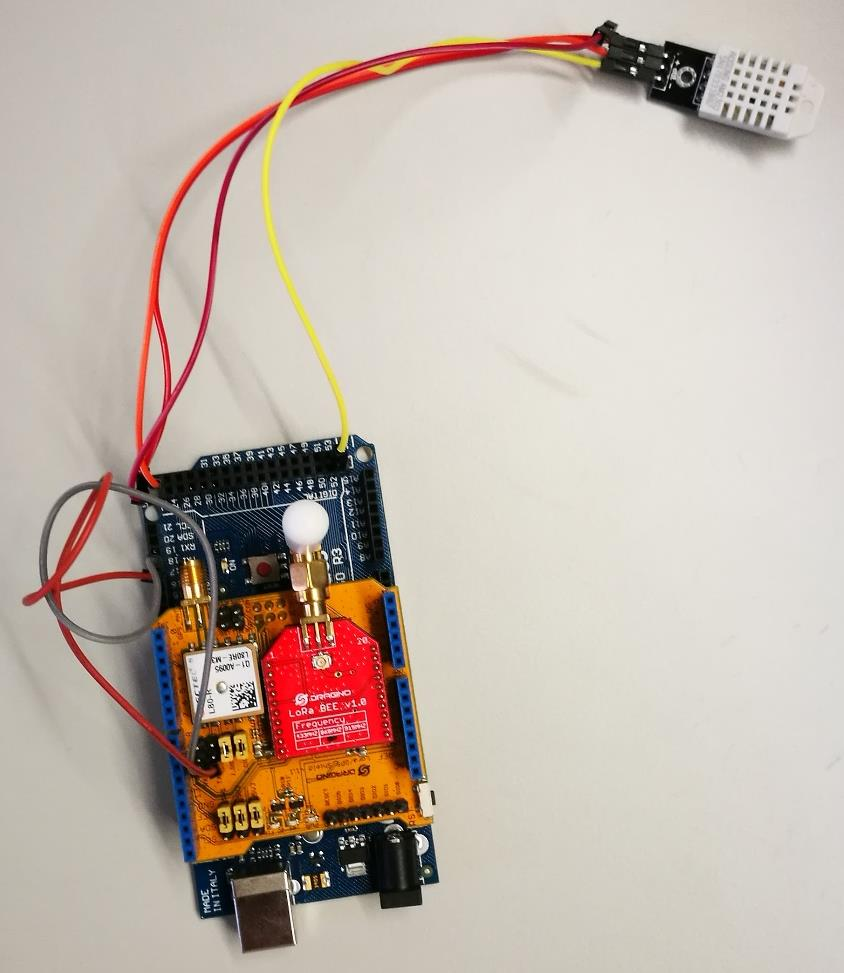
\includegraphics[width=0.2\textwidth]{figures/device}
\caption{Measurement device consisting of an Arduino Mega 2650 microcontroller with a Dragino GPS/LoRa shield. The depicted device also has a DHT22 temperature and humidity sensor.}
\end{figure}

The Arduino is programmed such that on start-up each minute a LoRa package is sent containing a counter variable as payload. The code is based Arduino-LMIC library\footnote{\url{https://github.com/matthijskooijman/arduino-lmic/}} and stores for each sent package the position and time data locally on an SD card. Initially the temperature and humidity was tracked as well by means of an DHT22 sensor (this was skipped later on). Table \ref{tab:dev} shows the first few lines of a device measurement file recorded on Dornbirn (Austria) November 2017. 

% latex table generated in R 3.4.3 by xtable 1.8-2 package
% Thu Jul 26 05:45:59 2018
\begin{table}[h!]
\centering
\begin{tabular}{rrrrrlrr}
  \hline
  counter & sat & lat & long & alt & time & H & T \\ 
  \hline
   0 &   4 & 47.41 & 9.75 & 413.80 & 11/24/2017 14:25:102766  & 40.00 & 13.60 \\ 
     1 &   4 & 47.41 & 9.75 & 413.80 & 11/24/2017 14:25:102766  & 40.00 & 13.60 \\ 
     2 &   4 & 47.41 & 9.75 & 413.80 & 11/24/2017 14:25:102766  & 40.00 & 13.60 \\ 
     3 &   4 & 47.41 & 9.75 & 448.20 & 11/24/2017 14:25:432297 & 40.80 & 13.60 \\ 
     4 &   4 & 47.41 & 9.75 & 457.40 & 11/24/2017 14:26:482383 & 41.30 & 13.60 \\ 
     5 &   5 & 47.41 & 9.74 & 459.50 & 11/24/2017 14:26:482383 & 41.10 & 13.00 \\ 
   \hline
\end{tabular}
\caption{Data that is stored on the field-test device: The \texttt{counter} variable denotes the payload. The GPS coordinates are stored in \texttt{lat}, \texttt{long} and \texttt{alt} where \texttt{sat} denotes the number of satellites.}\label{tab:dev}   
\end{table}

The device is registered in the TTN (\emph{the things network}) backend such that during the measurements each nearby TTN gateway receives the package containing the counter payload and forwards it to the TTN network server. There, the individual packages are merged and stored. Figure \ref{fig:topology} depicts the principle network scheme. 

\begin{figure}[h!]\label{fig:topology}
\centering
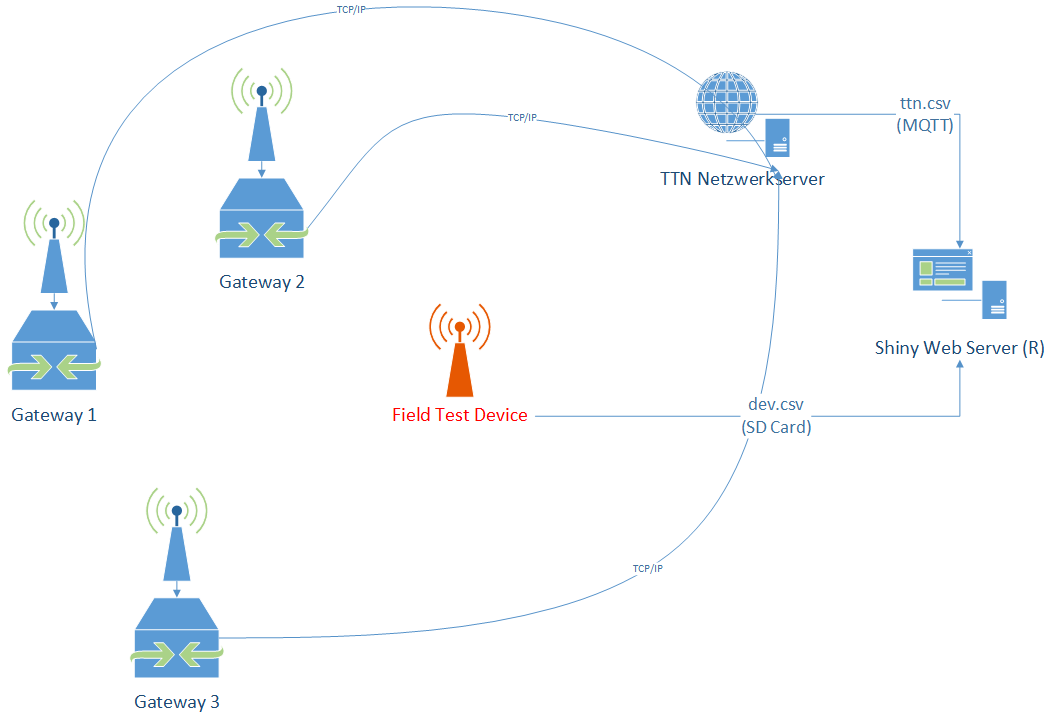
\includegraphics[width=0.8\textwidth]{figures/Topologie}
\caption{Network Topology to measure the RSSI/SNR for each position and gateway. The mobile device sends integer counters which are or are not received by the gateways. The send the RSSI and SNR values to the TTN network server. Here The web application subscribes via MQTT and receives the data. This data is then merged with the position and time data of the device. The interger counter serves as identifier.}
\end{figure}

When the measurement process is finished, the data from the network server is gathered by means of an MQTT request and stored on an application server that also hosts the web application (sc. Section \ref{sec:app}). In Table \ref{tab:ttn} the first few lines of such a data set is shown. The \texttt{counter} variable corresponds to the payload that was sent by the test device, i.e. it serves as a link between the test device (and its position) and the received data. The gateways are encoded by means of a unique ID (\texttt{gtw\_id}) provided by TTN. In Table \ref{tab:ttn}, for example, there are three gateways in total. The counter \texttt{0} appears two times, i.e. one gateway has lost the package. The package containing the payload \texttt{1} has been received by all gateways, where as the next package has been lost completely. For each received package the signal-to-noise ration \texttt{SNR} and the received signal strength indicator \text{rssi} are stored, which will be the basis of the statistical analysis introduced in Section \ref{sec:kriging}.


% latex table generated in R 3.4.3 by xtable 1.8-2 package
% Thu Jul 26 05:47:38 2018
\begin{table}[h!]
\centering
\begin{tabular}{rrllrrl}
  \hline
  counter &   gtw\_id & time & rssi & snr & dataRate \\ 
  \hline
     0 &   eui-1020304050607080 &  & -102 & 8.30 & SF7BW125 \\ 
     0 &   eui-9d4004f0211748e3 & 2017-11-24T14:24:37.339087Z & -91 & 8.80 & SF7BW125 \\ 
     1 &   eui-9d42000db93e82a5 & 2017-11-24T14:25:42.465766Z & -114 & 0.00 & SF7BW125 \\ 
     1 &   eui-9d4004f0211748e3 & 2017-11-24T14:25:42.455736Z & -109 & 3.20 & SF7BW125 \\ 
     1 &   eui-1020304050607080 &  & -107 & 8.30 & SF7BW125 \\ 
     3 &   eui-9d42000db93e82a5 & 2017-11-24T14:26:47.573741Z & -112 & 2.20 & SF7BW125 \\ 
     3 &   eui-9d4004f0211748e3 & 2017-11-24T14:26:47.566753Z & -89 & 9.80 & SF7BW125 \\ 
   \hline
\end{tabular}
\caption{Data file gathered from the TTN network server by means of an MQTT request. Each gateway has a unique ID, i.e. here three gateways have been in reach. The package with payload 2 has been lost for all gateways.}\label{tab:ttn}
\end{table}

On the application server the data file from the TTN backend is split up in separate tables for each gateway and these tables are then merged with the position information of the device by means of the counter variable. These tables are the basis of the statistical analysis in Section \ref{sec:kriging}


\section{Statistical Interpolation}\label{sec:kriging}

In this section we describe the proposed algorithm to produce an RSSI heat map. The basis for the heat map are the RSSI values measured for each gateway at different discrete positions for the field test device as shown in Figure \ref{fig:meas}. The blue marker in the Figure indicates the gateway position (here a gateway located at the \emph{Faulturm} in a purification plant in Dornbirn (Austria)). The red dots correspond to device positions where the color encodes the measured RSSI value. Obviously, close-by measurement points exhibit a larger RSSI value than more remote locations, however there are localized effects visible that can not be explained by the device-gateway distance only. Gray points belong to positions where the packages have been lost. 


\begin{figure}[h!]
\centering
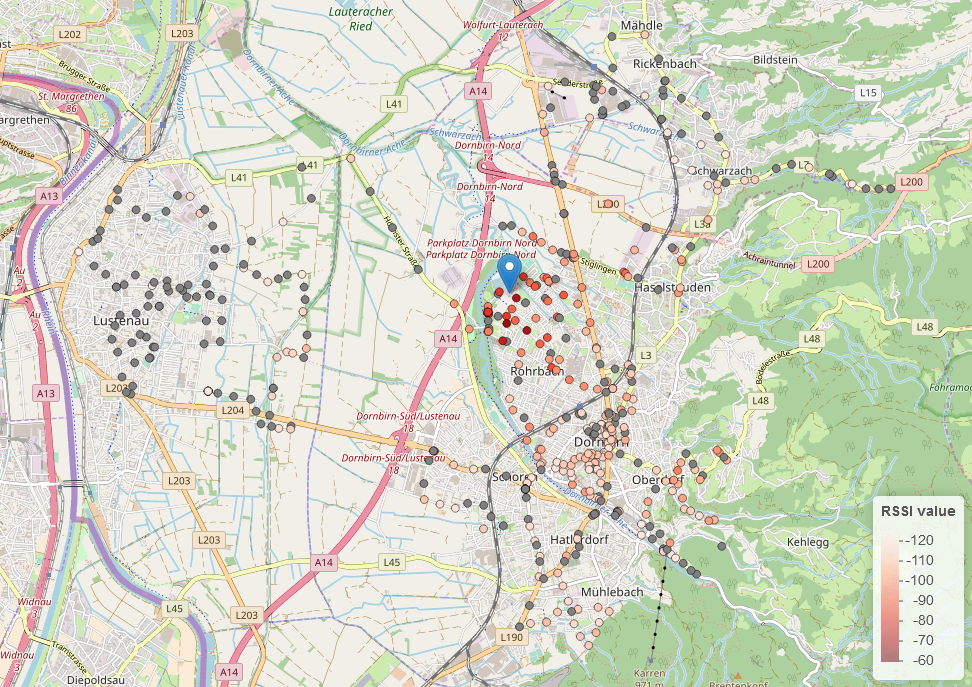
\includegraphics[width=0.7\textwidth]{figures/measurements}
\caption{Measurement positions in the Dornbirn area: The gateway (\emph{Faulturm}) is marked with the blue sign and the red dots correspond to measurements that were received by the gateway. The higher the RSSI value, the darker the red shade. Obviously close-by measurements exhibit a better RSSI value, however, there are also localized effects that can not be explained by the distance only. Gray dots indicated measurement positions with package loss.}\label{fig:meas}
\end{figure}

\begin{figure}[h!]
\centering
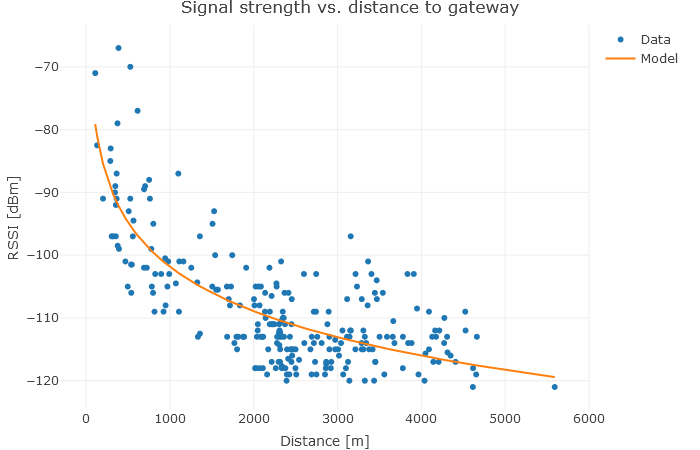
\includegraphics[width=0.7\textwidth]{figures/loglaw}
\caption{RSSI values vs. device/gateway distance for the \emph{Faulturm} gateway: The measurement values are shown as blue markers and the logarithmic model that was fitted to the data corresponds to the orange line.}\label{fig:law}
\end{figure}

\section{Web-App}\label{sec:app}

\section{Discussion}\label{sec:disc}

\bibliographystyle{abbrv}
\bibliography{literature}


\end{document}